% !TEX root = ../TechProject.tex

\graphicspath{{Chapter2/}}

\chapter{Machine Learning used in Music Recommendation Systems}

In this chapter Ill be answering the research question:

\textit{What are effective methods for the automated recommendation of songs suitable for adding to a given DJ set} 

\section{The need for music recommendation systems}
Spotify, SoundCloud, Apple Music and other streaming services gives one access to a library of tens of millions songs. Music Recommendation systems are excellent at fitting a user's preference whilst incorporating some level of filtering of an overwhelming amount of songs \citep{bollen_understanding_2010}. 

Music recommendation systems study the habits and tastes of users, and with that information give out suitable recommendations. This aids the listener to discover new songs or artists they otherwise would not have found.

With this potential, a well made recommendation system could be a make or break for choosing one stream service from another. For this reason a lot of research gets put into recommendation systems as an attempt to retain engagement. 

 With recommending music, a lot of sub conscious factors come into play on what a user wants to listen to at a given time. This can range from characteristics and mood of the listener \citep{ferwerda_personality_2015}  \citep{rentfrow_re_2003}, to what they get up to in day-to-day life \citep{gillhofer_iron_2015} \citep{wang_context-aware_2012}.  The users environment can have an affect as well \citep{kaminskas_location-aware_2013}. Observing a user made playlists also can reveal a lot on what groups of songs work for suited situations \citep{zheleva_statistical_2010} \citep{mcfee_hypergraph_2012}.
 
 A necessity for making a recommendation system suited for a type of product is taking into consideration the common place attributes of the product. Music lends itself to having a specific method due to short duration and high emotional connection. A recommendation system that uses these attributes to its advantage will be more successful than ones that don't.

\section{Collaborative filtering}

Collaborative filtering guesses a user's taste by looking at similar user-item connections. Using an explicit example, if a user rates something highly, it can provide similar suggestions from looking at the ratings of other users\citep{celma_recommendation_2010}.

\begin{figure}[H]
	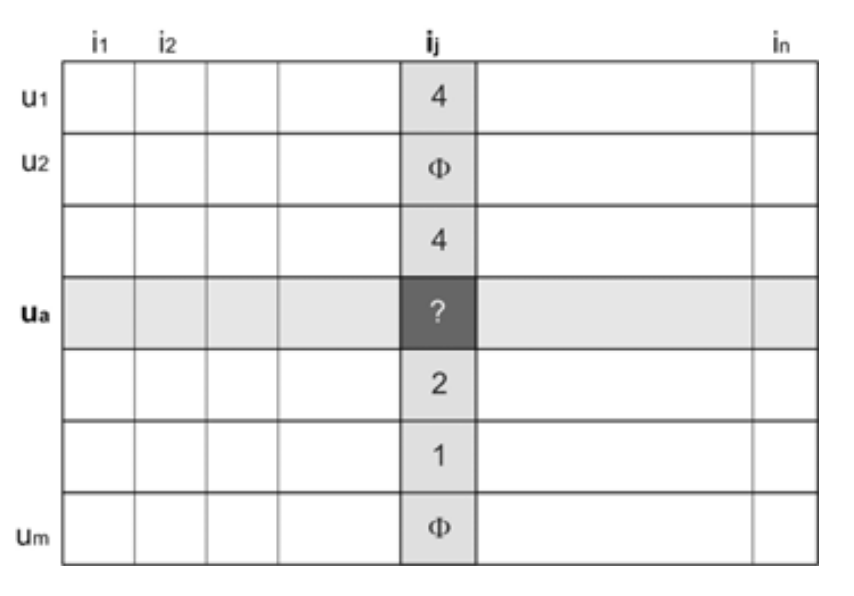
\includegraphics[scale=0.65]{images/collaborative_filtering}
	\centering
	\caption{User-item matrix used for collaborative filtering \citep{celma_recommendation_2010}} 
	\label{fig:figure}
\end{figure}

Collaborative filtering works by taking a matrix of users and items where some form of interaction is measured. Examples of interaction's could be plays of a song, rating of a movie/product or screen time on an app. In figure 2.1, i represents items, and u is users.

The first known use of collaborative filtering is with Goldberg's Tapestry system, a mailing list filter where users collectively decide which type of emails get the most importance \citep{goldberg_using_1992}. The first instance of collaborative filtering being used for music recommendations was in a system called \textit{Ringo} where users would rate music (album, songs, artists, etc.) and get recommendations pulled from similar users \citep{shardanand_social_1995}. 

Despite the prevalence of deep learning and neural networks, collaborative filtering is still used in today's state of the art recommendation systems. The winner of the 2018  RecSys Playlist Continuer Challenge used a combination of collaborative filtering and deep learning in their model \citep{volkovs_two-stage_2018}.

Collaborative filtering can be divided into the following types:

\begin{enumerate}
	\item Explicit Feedback
	\item Implicit Feedback
	\item Item Based
	\item User Based
\end{enumerate}




\subsection{Explicit Feedback}

\textit{Ringo} and many of the first music recommendation systems that use collaborative filtering uses explicit feedback for its data. Explicit feedback is when the system asks a user for some form of measurement about the likeability of said product. \citep{celma_recommendation_2010}

An example of explicit feedback being used is in the RACOFI (Rule-Applying Collaborative Filtering) system. Ratings are used to find recommendations through collaborative filtering and then the system applies logic rules to decipher the most suitable recommendations further \citep{anderson_racofi_2003}. Its added logic rules implicitly changes the user's previous ratings. Other recommendation systems started having similar rules including \textit{Indiscover} and Slope One \citep{celma_music_2010} \citep{lemire_slope_2007}.

\subsection{Implicit Feedback}

Recommendation systems that take only implicit feedback will focus on what the listener interacts with, rather than asking them for their opinion of the content. The main reason implicit feedback is frowned upon is that using this method doesn't give a scale of enjoyability of the content, in the context of music, just whether the user listened to said song or artist how many times. Spotify is an example of this, if another person uses their account or if they left a device on autoplay as well on mute. However, collecting implicit data is a lot easier because it just requires engagement with the said application to get valuable information. 

There is also a lot to be found with implicit data. In 2018, a music recommendation system produced effective recommendations derived from the time of day in which users listened to music \citep{sanchez-moreno_incorporating_2018}. Takama et al took this a step further by using time of day as well as, nationality and content features found through Spotify \citep{takama_context-aware_2021} 

\subsection{Item-Based Neighbourhood }

\textbf{Talk about the definitions and examples of these things \citep{ricci_recommender_2011}}

Item-Based Neighbourhood is when similarites for a given item is found based on the user's previous item ratings. Below shows a matrix with ratings from  $u_{2}, u_{i}$ and $u_{m-1}$. For finding similarities between $i_{i}$ and $i_{k}$, we only take $u_{2}$ and  $u_{i}$ into consideration when using item based neighbourhood because they have rated both item $i_{i}$ and $i_{k}$.  

\begin{figure}[H]
	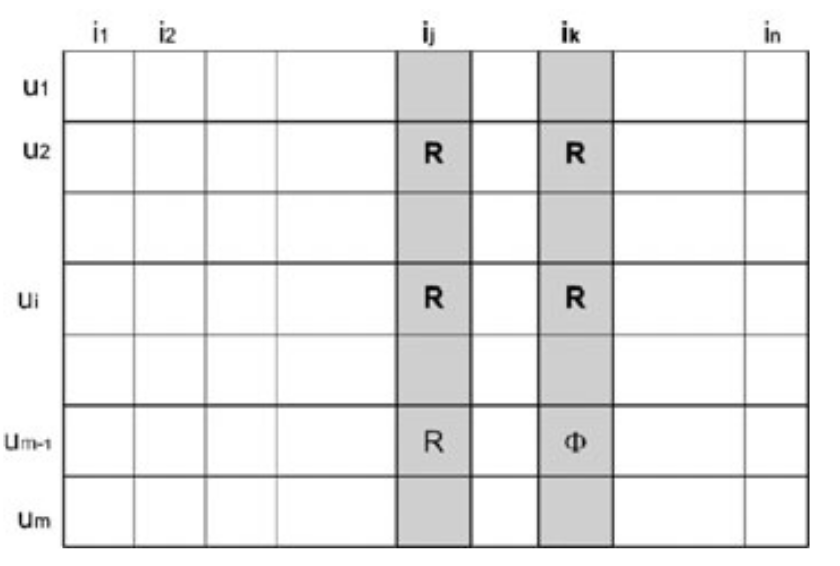
\includegraphics[scale=0.65]{images/neigbourhood_based}
	\centering
	\caption{Matrix showing given ratings. \citep{celma_recommendation_2010}} 
\end{figure}

There are many ways to calculate how similar two items, examples being cosine similarity, Pearson correlation or adjusted cosine similarity. For cosine similarity, the inner product space is taken into account by calculating its similarity, it can be described with the following equation.

\begin{equation}
		sim(i , j) = cos( \textbf{i}, \textbf{j} ) = \frac{ \textbf{ i }, \textbf{ j }}{ || i || * || j || } = \frac{ \sum_{ u \in U } r_{ u, i }, r_{ u, j }} { \sqrt{ \sum _{  u \in U } r^{2}_{ u , i}} \sqrt{ \sum _{  u \in U } r^{2}_{ u , j}}}
\end{equation}

Cosine similarity is not advised when comparing how similar recommendations are because users often have their own personal ranges when it comes to rating. Adjusted cosine similarity is good because it makes use of the users average ratings when deciphering similarities, the equation for adjusted cosine similarity is shown below.

\begin{equation}
	sim(i , j) = \frac{ \sum_{ u \in U } ( r _{ u, i } - \bar{r} _{u} ) ( r _{ u, j} - \bar{r} _{u} ) } { \sqrt{\sum_{ u \in U } ( r _{ u, i } - \bar{r} _{u} )^2} \sqrt{\sum_{ u \in U } ( r _{ u, j } - \bar{r} _{u} )^2}}
\end{equation}

Pearson correlation gives a coefficient value from 1 to -1, 1 showing strong correlation with a positive gradient, and -1 display effective correlation with a negative change.

\begin{equation}
	sim(i , j) = \frac{ Cov( i, j) }{ \sigma _{i} \sigma _{j} } = \frac{ \sum _{ u \in U} ( r _{ u, i } - \bar{r} _{u} ) ( r _{ u, j} - \bar{r} _{u} ) } { \sqrt{\sum_{ u \in U } ( r _{ u, i } - \bar{r} _{u} )^2} \sqrt{\sum_{ u \in U } ( r _{ u, j } - \bar{r} _{u} )^2}}
\end{equation}

After the similarities are calculated, the next step is to predict how the user would rate the item in question. A way of doing this is calculated a weighted sum of the users previous item ratings. Allowing $ S^{k}(i;u)$ to equal the list of items i user u has rated, equation below shows how the predicted value is found.

\begin{equation}
	\hat{r} _{u,i} = \frac{ \sum _{ j \in S^{k}(i;u)} sim(i , j) r _{u, j}}{\sum _{j \in S^{k}(i;u)} sim(i , j)}
\end{equation}




\subsection{User Based}

User-Based Neighbourhood is when you look users who rate similar to see whether item i is similar to user u. Below shows an equation similar to the one above but instead we look through a list similar users.

\begin{equation}
	\hat{r} _{u,i} = \bar{r}_{u} + \frac{ \sum _{v \in S(u)^{k}} sim(u ,v) ( r_{v, i} - \bar{r}_{v})}{\sum _{v \in S(u)^{k}} sim(u , v)}
\end{equation}

For one to calculate $sim(u , v)$, you'd use Pearson Correlation, Cosine similarity or matrix factorisation.

Item based is when the system predict rating of user u for item i rooted from ratings of u for similar items to i. Similarity between two items are affirmed when multiple users rate them alike.

\subsection{Matrix Factorisation}

Matrix factorisation is when you take a sparse matrix and instead of storing each rating for each user, you store features that when multiplied can calculate the rating of said item by said user.

This is really useful for a sparse matrix, which is usually the case for most recommendation systems, because it shows information that the matrix alone doesnt. Because it factorises the users ratings from features, you can see trends on what groups of users likes and doesnt like. Because it reducing the dimensionality of a given matrix, matrix factorisation requires less processing power than other methods of finding similar items. 

There are different ways of factorising a matrix. An example of one is Singular Value Decomposition (SVD). Heres the equation with U and V being the number of matrices for a given amount dimensions:

\begin{equation}
	M = U \sum V ^{T}
\end{equation}

Theres other means to compute M. Least Squares, uses a computational safe way to make sure M doesnt go to off from its original value, whilst stochastic gradient repetitively uses random bits of data to approximate U and V \citep{koren_matrix_2009}. 

When the matrix is split up, the predicted rating can be calculated from the user and item feature vectors. 

\begin{equation}
	\hat{r} _{u,i} = U _{u} . V _{i}^{T} = \sum_{f=0}^{k} U_{u,f} V_{f, i}
\end{equation}

Looking at the latent factors one can find  similar items using a cosine similarity.

\subsection{Limitations}
Despite being popular, there are a number of reasons why wouldn't use Collaborative filtering.

\textbf{Sparse Data - }Not every user has listened to every song, far from it. This means in data sets, having a sparsity of around 98-99 \% is very common.

\textbf{Grey sheep - }This is when a user has a unique taste not similar to a lot of other users, making it hard to stem recommendation's from. This a common problem with datasets that are very sparse \citep{claypool_combining_1999}.

\textbf{Cold Start - } When there is new users or items, theres little data associated with them so it makes it challanging to come up with suitable mendations based on either the said user or item. The term cold start refers to new items and the term refered to new users is called early raters \citep{avery_recommender_1997}.

\textbf{Popularity Bias - } Another problem with Collaborative Filtering doesnt take into account any information about the item, only users interactions with it. This means that it has a bias towards popular items.

\textbf{Feedback loops - } When users interact with items that are recommended through CF, based on previous user item interactions, it strengthens the initial recommendations more and creates a loop \citep{sanchez-moreno_incorporating_2018}.


For neighbourhood-based, recommendation can either be user-based or item-based. The Ringo system is a good example of user based recommendation's, where it assesses the taste of a user for an item using the ratings of the item from different users. These users with similar rating trends are called neighbours. 

\textbf{Talk about latest music mendation system that uses it (recsys one)}
\section{Content Based Filtering}

Content Based Filtering works by looking at the characteristics of a given item and see if it matches the preference of the user. Recommendations do not stem from what other users interact with, it only stems from the given information about the item. Its based on finding information about the item and filtering \citep{casey_content-based_2008}, and within the context of music, it recommends songs that has similar information to what the user already enjoys \citep{aucouturier_music_2002} \citep{logan_music_2004}. Theres been a lot of research on extracting the componenets of an audio file of music \citep{ribecky_multi-input_2021} \citep{zhao_musical_2022}. Recent developments have shown successful extractions of genre and structure with the MusicBERT Model \citep{zhu_musicbert_2021}. It's found that midi extraction from songs can aid to give better solutions for less popular songs, helping eliminate the cold start problem \citep{yadav_improved_2022}.

Early uses of content based filtering were text based, because of its ease of information extraction, An example of this is the PRES system \citep{van_meteren_using_2000}. But now with advances in machine learning, more complex formats can be used for extraction like images or audio. Models like "Xception" have proven successful at extracting audio features from songs \citep{chollet_xception_2017} \citep{singh_robustness_2022}.

When finding similar items with CB, it simply looks at how similar the attributes of each items is, without introducing any subjective factor, like user behaviour, into its decision making. Thinking of an item being a vector made of its defined values of attributes, we can find the distance between each item. Its common to have these values be numerical. Common ways of caluclating the distance is Euclidean, Manhattan, Chebychev, cosine distance for vectors, and Mahalanobis distance.

\begin{equation}
	d(x,y) = \sqrt{\sum _{i=1} ^{n}(x_{i} - y_{i})^{2}}
\end{equation}

\begin{equation}
	d(x,y) = \sum _{i=1} ^{n} | x_{i} - y_{i} |
\end{equation}

\begin{equation}
	d(x,y) = man_{i} = _{1 . . n} | x_{i} - y_{i} |
\end{equation}

\begin{equation}
	d(x,y) = \sqrt{ ( x - y )^{ T } S^{ -1 } ( x - y ) }
\end{equation}

Euclidean, Manhattan and Chebychev distance are used when there is little relationship or correlation between attributes. If there is correlation, its advised to use Mahalanobis distance \citep{celma_recommendation_2010}.

When the attributes aren't measured numericlly, one uses a delta function. When two attributes match it equals zero, other wise it equals 1.

\begin{equation}
	d(x,y) = \omega \sum _{ i = 1 } ^{ n } \delta (x _{i}, y _{i})
\end{equation}

Content Based Filtering overcomes the problems CF has of being able to rate items that previously havent had any ratings. Its also able to adapt to any changes in the users preference quickly \citep{isinkaye_recommendation_2015}. For users who dont want to share there data they can get suitable mendations as well \citep{k_you_2006}.

Another methods of comparing includes Clustering. Clustering is when one  groups a collection of data objects, so that some objects clustered together are very similar, while other clustered objects are not alike. Similarity is then evaluated based on chosen parameters \citep{ferretti_clustering_2018}. A popular algorithm is the k-mean cluster where each cluster is representerd by a mean value of the object \citep{han_data_2006}. A recent system that uses clustering uses a altered version to k clustering to limit the randomness in suggestion you usually get with this method \citep{chang_personalized_2017}.



\subsection{Limitations}
The cold start and grey sheep problem also occur in content based filtering. It's often the case where popular items would have better defined features, and older users well have better represented features.

\textbf{Novelty Problem - } This is when the user is recommended items too similar to the one there profile, an application would need some way of diversifying recommendations to overcome this.

\textbf{Retrieving metadata - } Even though we have seen recent improvements in extracting meaningful meta data \citep{vall_feature-combination_2019} \citep{singh_novel_2022}. One uses this data in deep neural networks or hybrid models. We aren't yet at a point where we can obtain rich enough meta data to rely on Content Based Filtering alone.

\textbf{Suggestions not opinionated- } It doesn't take into the account the opinions of users, only description of what the item is. This may lead to some poor quality recommendations.  


\section{Diversity issue}

Recommendation systems are used extensively by majority of spotify users. However, there are a subsection of users who, despite huge breakthroughs dont rely heavily on algorithmic means of discovering music. In 2020, there was a study done that found users with more diverse tastes would find music in non algoritmic ways \citep{anderson_algorithmic_2020}. This study also found state of the art mendation systems performed better with users with less diverse taste. and users who would gain a more diverse taste over time, would do so by exploring non algorithmic ways of finding music.

A reason for this is because alogorithmic ways go above and beyond giving personalised suggestions, one can suffer from choice overload when using algorithmic ways to find music \citep{iyengar_rethinking_1999}. This may do with the lack of refinement when it comes to training models, lot of MRS dont focus on a specific type of person when training a model \citep{laplante_improving_2014}.

A reason for this issue could be the way classification is handled in music mendation systems, a debate that is passed from generations \citep{moles_sociodynamique_2019} \citep{dimaggio_classification_1987} \citep{bourdieu_distinction_2010}. In the context of a mndation system, a genre is usually just treated as a "tag" and its social and cultural relevance is often pushed to the side when treated in such a way \citep{porcaro_diversity_2021}. The act of a machine understanding a intensely subjective concept as genre is one that is proven challenging \citep{nurnberger_survey_2014}. Vlegels attempts to overcome this by organise groupings based on user artist relationship, rather than artists genre \citep{vlegels_music_2017}.

This problem itself has saw another rise in the market of "curation". Having professional spot interesting things and document them to consumers. With this comes the role in the music world of a DJ, who way before recommendation systems existed were doing just that. Recently we have seen attempts of integrating DJs somehow in the algorithmic world. This is partly motivated by how much a company can pedel a term like "curation" in the music world and see it as a necessity \citep{barna_perfect_2017}. One can see this in the rise of internet radio as well.

Internet Radio is a strangely thriving industry which is expected to have an net worth of 9.2\$ billion \citep{market_research_future_internet_2022}. There are many different factors on why this resurgence has occurred on a platform that one could easily see die. The quoted figure would also include radio beyond the scope of music. But specifically in dance music centric radio has also received a huge rise \citep{gillett_how_2021}. It includes increased speeds in mobile data, and the choice of stations, but one can see the push for curation from leading companies in this field \citep{deane_media_apple_2020} \citep{nts_radio_nts_2023}.

The closest integration we got with DJ's and the algorithmic centric streaming apps is Apple Musics Beats 1 Radio station where apart of the subscription service you got access to a radio station of the most popular artist and DJs in the western world broadcasting shows, providing entertaining commentary and selected musical recommendations. Another is spotifys curated playlists, and more specifically there track ID's series, where they get established DJs to make a huge ever changing playlist of songs they play out live. The only instance I found of combining the two is a medium article written by Daniel Chow where he made a recommendation system out of the many DJ mixes found on mixesDB which takes in a single song and looking through the dataset find similar songs \citep{chow_music_2020}. Within the context of a DJ set finding recommendationd from multple songs, or a whole other set is something that has been previously unexplored, and could provide with solutions with assuring a exciting level of diversity that is missed in many recommendation systems.

% note that \Blindocument has 5 numbered levels, despite setting secnumdepth above. I (and many style guides) would suggest using no more than 3 numbered levels (incl. the chapter), with the option of a fourth unnumbered level.